\begin{figure}[H]
\centering
\includegraphics[page=6,width=0.33\textwidth]{\FCNCFigures/tthML/showFake/faketau/postfit/NOMINAL/reg1l2tau1bnj_os/BDTG_test.pdf}
\put(-40, 90){\textbf{(a)}}
\includegraphics[page=6,width=0.33\textwidth]{\FCNCFigures/tthML/showFake/faketau/postfit/NOMINAL/reg1l2tau1bnj_os/dphitauetmiss.pdf}
\put(-40, 90){\textbf{(b)}}
\includegraphics[page=6,width=0.33\textwidth]{\FCNCFigures/tthML/showFake/faketau/postfit/NOMINAL/reg1l2tau1bnj_os/drlbditau.pdf}
\put(-40, 90){\textbf{(c)}}
\\
\includegraphics[page=6,width=0.33\textwidth]{\FCNCFigures/tthML/showFake/faketau/postfit/NOMINAL/reg1l2tau1bnj_os/drlb.pdf}
\put(-40, 90){\textbf{(d)}}
\includegraphics[page=6,width=0.33\textwidth]{\FCNCFigures/tthML/showFake/faketau/postfit/NOMINAL/reg1l2tau1bnj_os/drltau.pdf}
\put(-40, 90){\textbf{(e)}}
\includegraphics[page=6,width=0.33\textwidth]{\FCNCFigures/tthML/showFake/faketau/postfit/NOMINAL/reg1l2tau1bnj_os/drtaub.pdf}
\put(-40, 90){\textbf{(f)}}
\\
\includegraphics[page=6,width=0.33\textwidth]{\FCNCFigures/tthML/showFake/faketau/postfit/NOMINAL/reg1l2tau1bnj_os/drtaujmin.pdf}
\put(-40, 90){\textbf{(g)}}
\includegraphics[page=6,width=0.33\textwidth]{\FCNCFigures/tthML/showFake/faketau/postfit/NOMINAL/reg1l2tau1bnj_os/drtautau.pdf}
\put(-40, 90){\textbf{(h)}}
\includegraphics[page=6,width=0.33\textwidth]{\FCNCFigures/tthML/showFake/faketau/postfit/NOMINAL/reg1l2tau1bnj_os/etamax.pdf}
\put(-40, 90){\textbf{(i)}}
\\
\includegraphics[page=6,width=0.33\textwidth]{\FCNCFigures/tthML/showFake/faketau/postfit/NOMINAL/reg1l2tau1bnj_os/etmiss.pdf}
\put(-40, 90){\textbf{(j)}}
\includegraphics[page=6,width=0.33\textwidth]{\FCNCFigures/tthML/showFake/faketau/postfit/NOMINAL/reg1l2tau1bnj_os/lep_pt_0.pdf}
\put(-40, 90){\textbf{(k)}}
\includegraphics[page=6,width=0.33\textwidth]{\FCNCFigures/tthML/showFake/faketau/postfit/NOMINAL/reg1l2tau1bnj_os/met_sigma.pdf}
\put(-40, 90){\textbf{(l)}}
\\
\caption{ The variables distributions for the background and merged tuH signal in the $l\thadhad$}
\label{fig:var_reg1l2tau1bnj_os_1}
\end{figure}
\begin{figure}[H]
\centering
\includegraphics[page=6,width=0.33\textwidth]{\FCNCFigures/tthML/showFake/faketau/postfit/NOMINAL/reg1l2tau1bnj_os/mjjmin.pdf}
\put(-40, 90){\textbf{(a)}}
\includegraphics[page=6,width=0.33\textwidth]{\FCNCFigures/tthML/showFake/faketau/postfit/NOMINAL/reg1l2tau1bnj_os/mtaujmin.pdf}
\put(-40, 90){\textbf{(b)}}
\includegraphics[page=6,width=0.33\textwidth]{\FCNCFigures/tthML/showFake/faketau/postfit/NOMINAL/reg1l2tau1bnj_os/mtw.pdf}
\put(-40, 90){\textbf{(c)}}
\\
\includegraphics[page=6,width=0.33\textwidth]{\FCNCFigures/tthML/showFake/faketau/postfit/NOMINAL/reg1l2tau1bnj_os/nljet.pdf}
\put(-40, 90){\textbf{(d)}}
\includegraphics[page=6,width=0.33\textwidth]{\FCNCFigures/tthML/showFake/faketau/postfit/NOMINAL/reg1l2tau1bnj_os/phicent.pdf}
\put(-40, 90){\textbf{(e)}}
\includegraphics[page=6,width=0.33\textwidth]{\FCNCFigures/tthML/showFake/faketau/postfit/NOMINAL/reg1l2tau1bnj_os/t1vismass.pdf}
\put(-40, 90){\textbf{(f)}}
\\
\includegraphics[page=6,width=0.33\textwidth]{\FCNCFigures/tthML/showFake/faketau/postfit/NOMINAL/reg1l2tau1bnj_os/t2vismass.pdf}
\put(-40, 90){\textbf{(g)}}
\includegraphics[page=6,width=0.33\textwidth]{\FCNCFigures/tthML/showFake/faketau/postfit/NOMINAL/reg1l2tau1bnj_os/tau_pt_0.pdf}
\put(-40, 90){\textbf{(h)}}
\includegraphics[page=6,width=0.33\textwidth]{\FCNCFigures/tthML/showFake/faketau/postfit/NOMINAL/reg1l2tau1bnj_os/tau_pt_1.pdf}
\put(-40, 90){\textbf{(i)}}
\\
\includegraphics[page=6,width=0.33\textwidth]{\FCNCFigures/tthML/showFake/faketau/postfit/NOMINAL/reg1l2tau1bnj_os/tautauvispt.pdf}
\put(-40, 90){\textbf{(j)}}
\includegraphics[page=6,width=0.33\textwidth]{\FCNCFigures/tthML/showFake/faketau/postfit/NOMINAL/reg1l2tau1bnj_os/ttvismass.pdf}
\put(-40, 90){\textbf{(k)}}
\caption{ The variables distributions for the background and merged tuH signal in the $l\thadhad$}
\label{fig:var_reg1l2tau1bnj_os}
\end{figure}
